\documentclass[11pt,a4paper]{article}
\usepackage[margin=2.2cm]{geometry}
\usepackage[T1]{fontenc}
\usepackage{lmodern,microtype,amsmath,graphicx,float,hyperref,parskip}
\graphicspath{{figures/}}
\title{Copper Certificate Valuation\\\large Results, Method and Operational Status}
\author{Mohammadmahdi Amirabadi}
\date{26 September 2026}
\begin{document}
\maketitle
\section{Purpose and delivered result}
The objective is to measure the copper certificate premium or discount to comparable
domestic physical copper. This is the primary output. Two independent comparisons
with intrinsic value provide context, not substitutes for the main measure.
The valuation product is complete and supports routine updates. Earlier investigations
of producers, trading gaps and alternative models supported this calculation.
The global copper/COCHILCO study is a separate project.

\section{Sources and method}
Certificate settlement prices and physical cathode transactions come from the Iran
Mercantile Exchange. LME cash quotations are collected through Westmetall. USD/IRR
uses the shared TGJU-derived history and its labeled legacy observations.
The physical benchmark is quantity-weighted eligible NCI cathode trading under the
approved cash and cash-matching scope. Intrinsic value in IRR/kg is
\[I_t=(LME^{cash}_t/1000)FX_t.\]
LME and FX use the latest observation on or before the target date. At jointly
observed certificate/physical dates, the physical-to-intrinsic ratio is measured.
Between anchors, this ratio is interpolated by calendar day and multiplied by
contemporaneous intrinsic value to estimate physical price. No extrapolation
before the first or after the last anchor is used.

\section{Primary result: certificate versus physical}
\[B^{C/P}_t=100(C_t/\widehat P_t-1).\]
Positive values indicate a premium and negative values a discount. Physical value
is observed at anchors and estimated between them. This is the main chart and
the source of the Power BI delivery table.
\begin{figure}[H]\centering
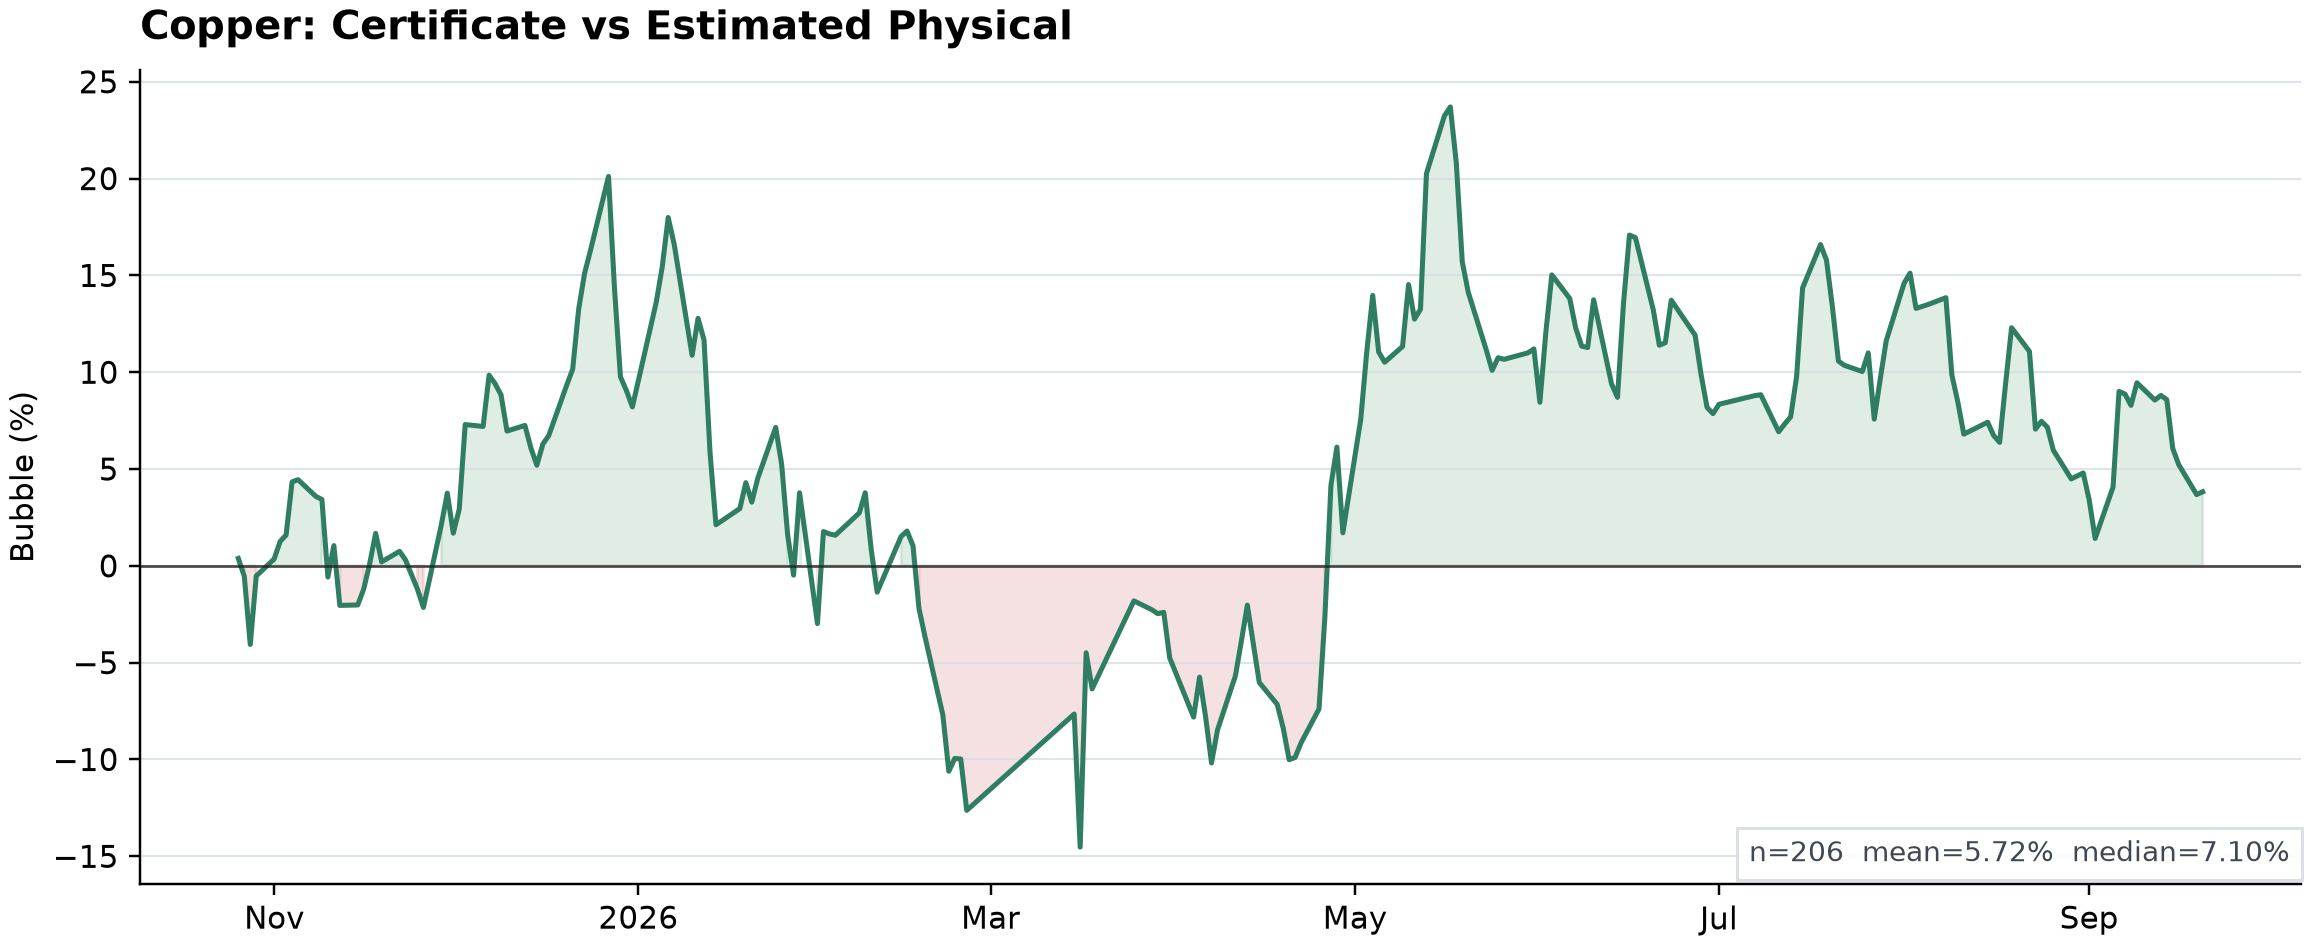
\includegraphics[width=\textwidth]{copper_main_bubble.png}
\caption{Primary comparison: certificate versus estimated domestic physical value.}
\end{figure}

\section{Supporting result: certificate versus intrinsic}
\[B^{C/I}_t=100(C_t/I_t-1).\]
This measures the certificate against the international-price and exchange-rate reference.
\begin{figure}[H]\centering
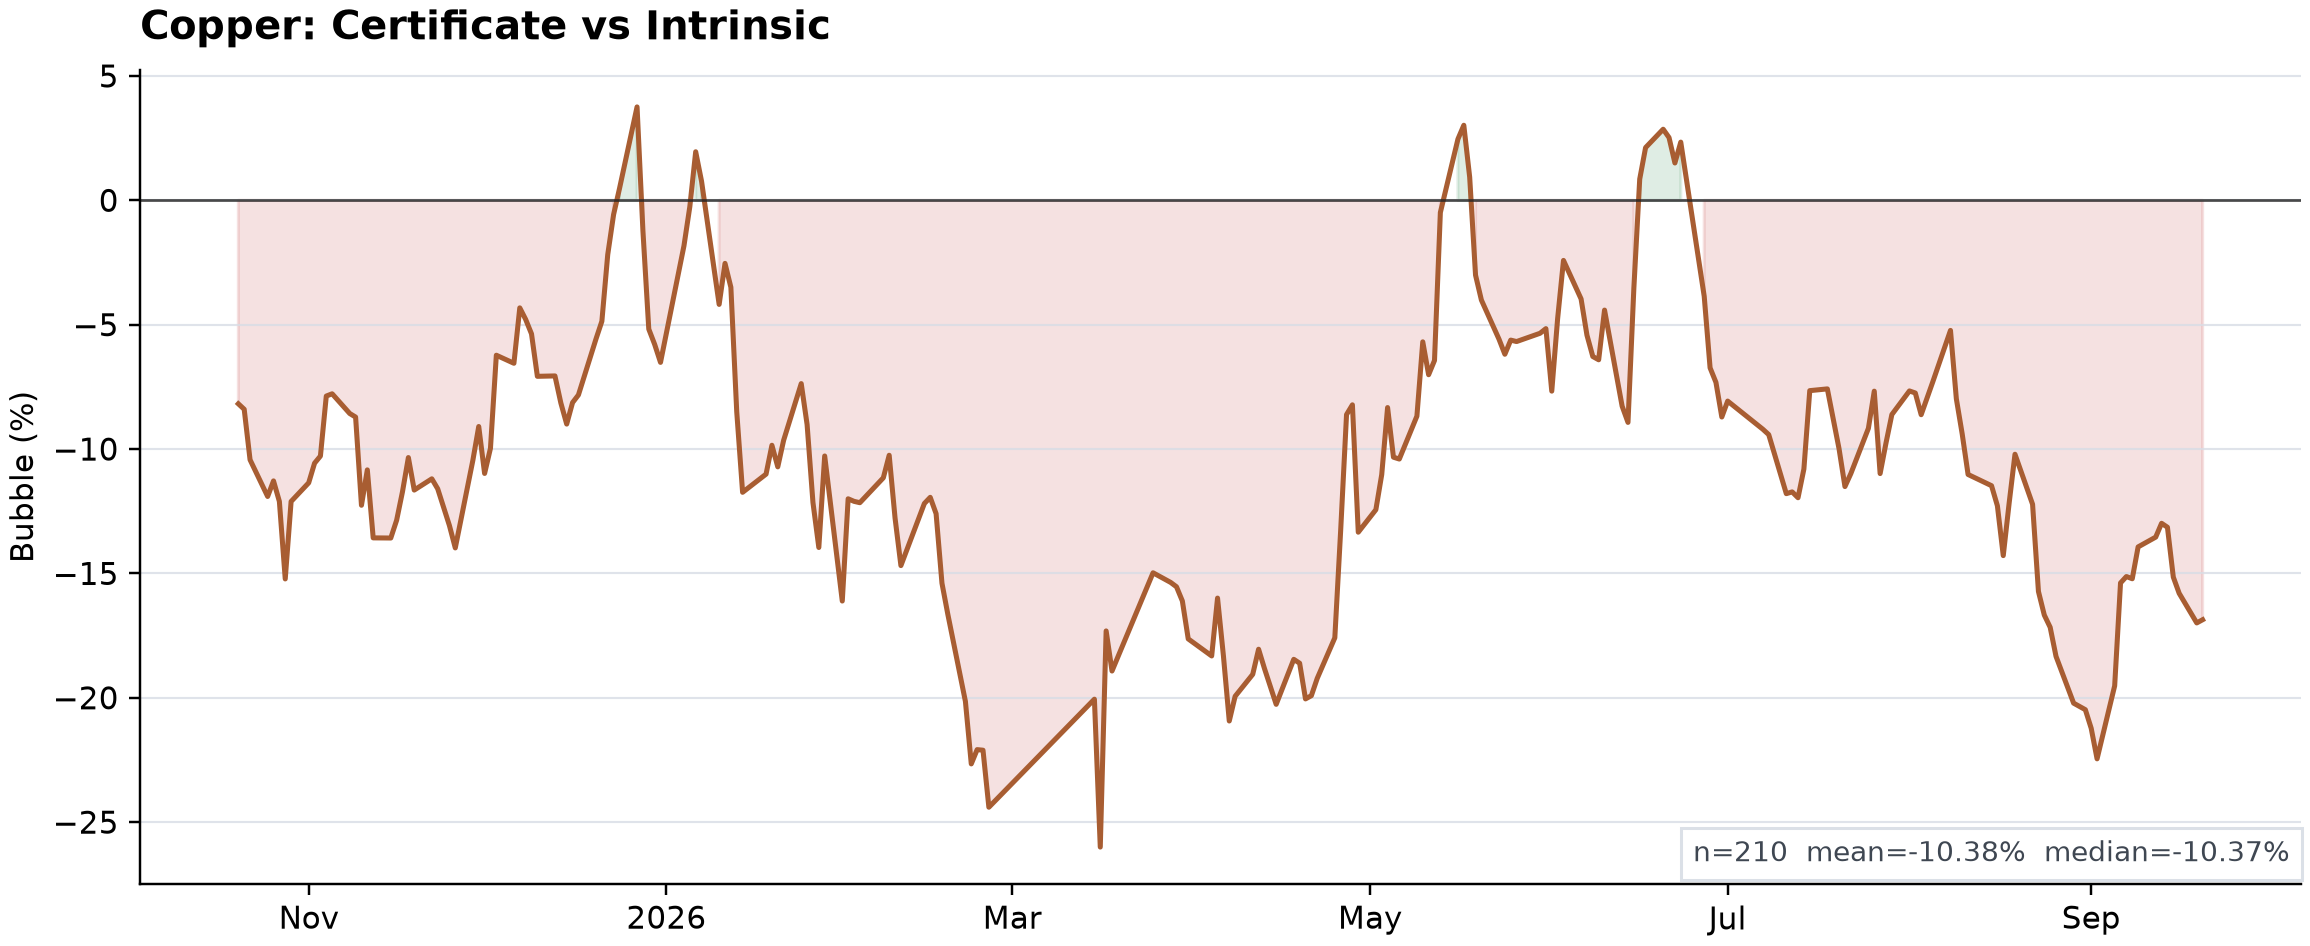
\includegraphics[width=\textwidth]{copper_certificate_bubble.png}
\caption{Supporting comparison: certificate versus intrinsic value.}
\end{figure}

\section{Supporting result: physical versus intrinsic}
\[B^{P/I}_t=100(P_t/I_t-1).\]
This measures the domestic physical basis on observed physical-trading dates.
The series have different coverage; a negative intrinsic comparison can coexist
with a positive certificate-to-physical premium.
\begin{figure}[H]\centering
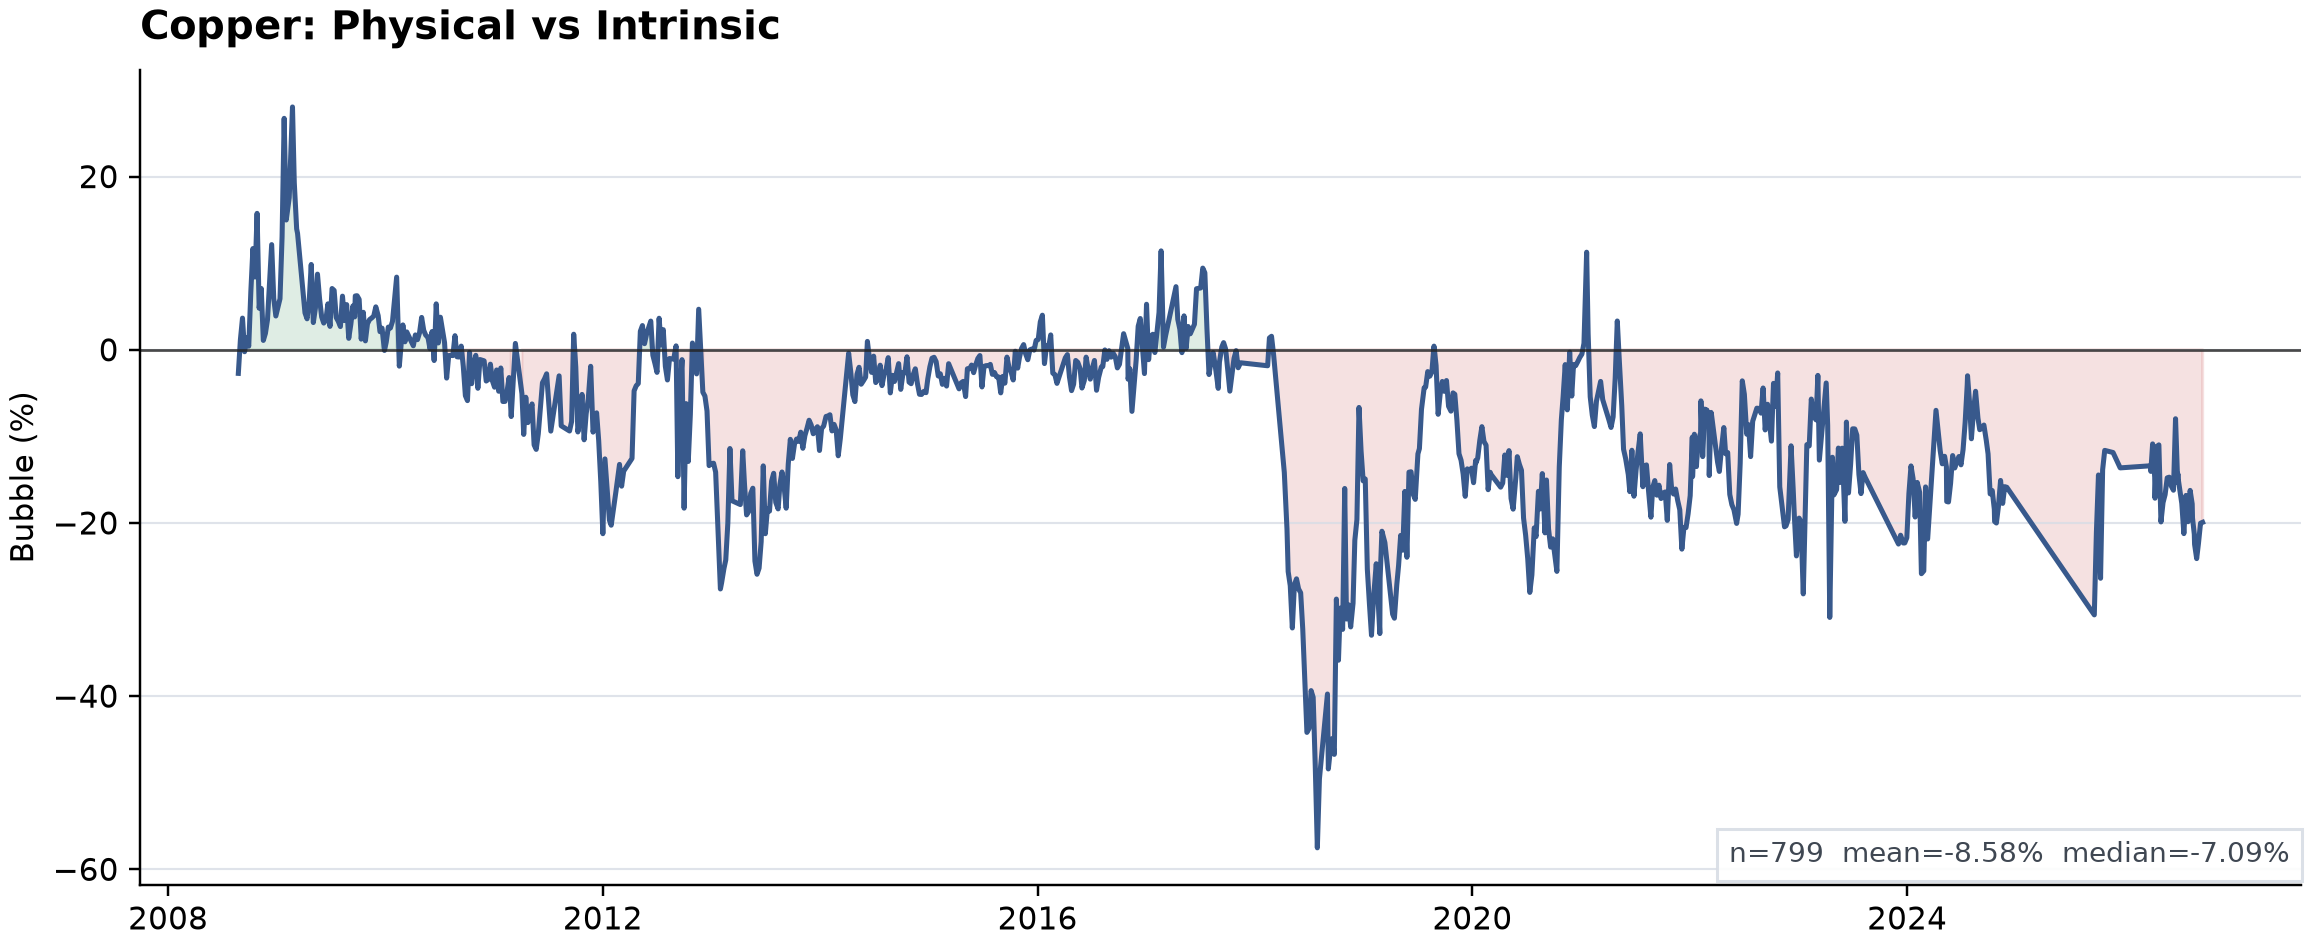
\includegraphics[width=\textwidth]{copper_physical_bubble.png}
\caption{Supporting comparison: observed physical versus intrinsic value.}
\end{figure}
Dates and numerical annotations in these charts are generated from processed
inputs rather than maintained as fixed figures in the report prose.

\section{Outputs and routine updates}
The production workflow builds the physical benchmark, three approved comparisons,
their distribution table and the Power BI export. Shared input preparation provides
one implementation of alignment and intrinsic value. The exporter transfers the
canonical result; recalculation only checks consistency.
From the workspace root:
\begin{verbatim}
python commodity/copper/refresh_powerbi.py
python reports/copper/research/build_figures.py
\end{verbatim}
The first command uses local data; add \texttt{--collect} to fetch source updates.
The second refreshes report charts. Compile this file from its own directory.
Experimental regression, the historical forward-gap study and presentation timelines
are retained research outputs, not routine deliverables. They require explicit
refreshes and must not be assumed current merely because their CSV files exist.
See the project's \texttt{docs/OUTPUTS.md} for ownership and refresh commands.

\section{Interpretation}
This is a historical relative-price estimate, not guaranteed tradable arbitrage.
Interpolation uses surrounding anchors, including a later anchor, so it is not
a real-time forecast or look-ahead-free backtest signal. Intrinsic value excludes
domestic carrying, delivery and transaction costs. These distinctions do not
alter the completed status of the calculation product.
\end{document}
